\documentclass[12pt, a4paper]{article}
\usepackage[UTF8]{ctex}
\usepackage{amsmath}
\usepackage{amssymb}
\usepackage{amsthm}
\usepackage{geometry}
\usepackage{enumitem}
\usepackage{indentfirst}
\usepackage{caption}
\usepackage{fancyhdr}
\usepackage{booktabs}
\usepackage{titlesec}
\usepackage{draftwatermark}%水印
\usepackage{graphicx} % 导入图像的宏包、单图
% 页面布局设置
\geometry{top=2.54cm, bottom=2.54cm, left=3.18cm, right=3.18cm}

\SetWatermarkText{B站：布加拉提}
\SetWatermarkScale{0.4}

% 行距设置
\linespread{1.5}

% 段落设置
\setlength{\parindent}{2em}
\setlength{\parskip}{0.5em}

% 节标题格式设置
\titleformat{\section}{\normalfont\Large\bfseries}{第\chinese{section}章、}{1em}{}
\titlespacing{\section}{0pt}{2.5ex plus 1ex minus .2ex}{1.3ex plus .2ex}

% 定理环境设置
\newtheoremstyle{solution}
{}
{}
{}
{}
{\bfseries}
{、}
{1em}
{}
\theoremstyle{solution}
\newtheorem{sol}{解}

% 页眉页脚设置
\pagestyle{fancy}
\fancyhf{}
\fancyhead[C]{b站布加拉提整理（回忆版）b站甘茶w独家讲解}
\fancyfoot[C]{\thepage}

\rfoot{整理人：八方\\资源提供：考研乔瑟夫}
\lhead{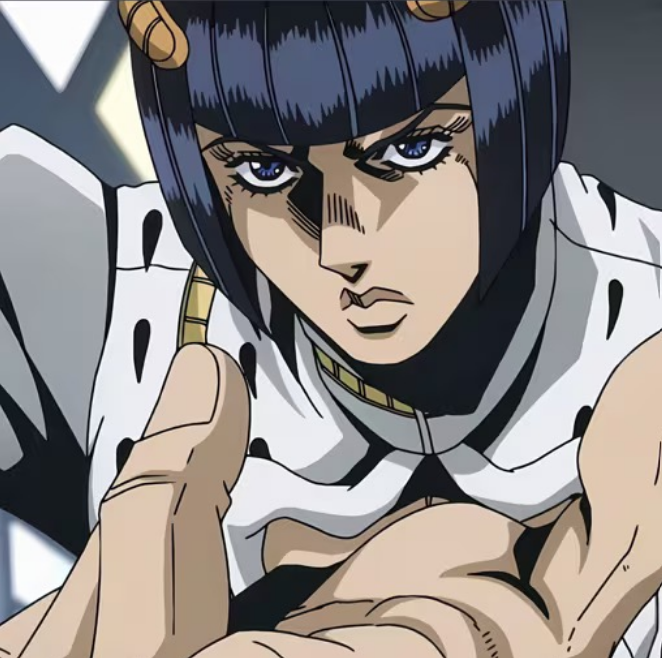
\includegraphics[width=0.06\linewidth]{p1.png}}
\rhead{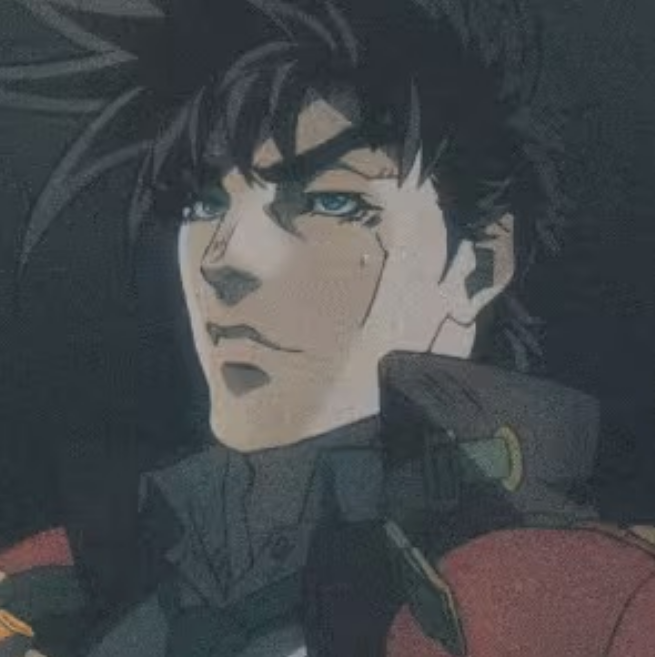
\includegraphics[width=0.06\linewidth]{p2.png}}
\renewcommand{\headrulewidth}{0.4pt}
\renewcommand{\footrulewidth}{0.4pt}

\begin{document}

\begin{center}
\Large\textbf{2022哈工大硕士考试试题：805物理光学}
\end{center}





\section*{一、选择题}
\begin{enumerate}
    \item 两块平板玻璃构成劈尖，左边为棱边，用单色平行光垂直入射，若上面的平板玻璃以棱边为轴，沿咩（模糊）方向做微小转动，则干涉条纹\_\_\_\_\_。
    \item （重复）单色平行光垂直照射在光学薄膜上，经上下两个表面反射的两束光发生干涉，若薄膜的厚度为 $h$，$n_1,n_2,n_3$相应为入射介质，薄膜和基底材料的折射率，且 $n_1<n_2>n_3$，$\lambda_1$为入射光在$n_1$，中的波长，则两束反射光的光程差为\_\_\_\_\_.
    A.$2n_2h-\lambda_1/2n_1$ \quad B.$2n_1h$ \quad C.$2n_2h-n_1\lambda /2$ \quad D.$2n_2h-n_2\lambda_1/2$ \quad
    \item 在双缝干涉实验中，为使屏上的干涉条纹间距变大，可采取的办法是\_\_\_\_\_。
    A.使屏靠近双缝\quad B.使两缝间距变小\quad C.把两缝的宽度稍微调窄\quad D.改用波长较小的单色光源
    \item $x=d \lambda/f$三个选项是公式里的字母，还有一个错误选项是衍射级次。
    \item 某一波长真空为1，则在长度为d，折射率为n的介质中的相位差为\_\_\_\_\_.
    \item 牛顿环从内到外的颜色\_\_\_\_\_。
    \item 表征光波是横波的性质\_\_\_\_\_。
    A.偏振\quad B.衍射\quad C.干涉\quad D.色散
    \item 给频谱宽，问相干长度，时间
    \item 01年1.1，04年1.4
\end{enumerate}
\section*{二、填空题}
\begin{enumerate}
    \item 两列相干波的振幅比$A_1/A_3=3$时，条纹对比度为\_\_\_\_\_，$A_1/A_3=3$=\_\_\_\_\_时，条纹最清晰。
    \item 氪同位素的橙黄色谱线$\lambda=605.7802nm$，谱线宽度$\Delta V=384MHZ $，其相干长度为\_\_\_\_\_，相干时间为\_\_\_\_\_。
    \item 迈克尔逊移动$\Delta H$变化\_\_\_\_\_，级次变化2048个条纹。
    \item 菲涅尔公式表示反射光，折射光，入射光\_\_\_\_\_和\_\_\_\_\_的关系，写出反射系数\_\_\_\_\_，\_\_\_\_\_。
\end{enumerate}
\section*{三、名词解释}
\begin{enumerate}
    \item 古斯-哈恩斯位移
    \item 倏逝波电光效应
    \item 群速度
    \item 条纹对比度
    \item 双折射
\end{enumerate}
\section*{四、简答题}
\begin{enumerate}
    \item 简述瑞利散射的特点
    \item 望远镜，显微镜，照相机物镜的分辨率，如何提升？
    \item 光波在金属表面反射与玻璃表面反射相比，反射有什么特点？
    \item 条纹可见度与什么因素有关？
    \item 比较棱镜与光栅的色分辨本领的区别？
    \item （重复）什么是旋光效应？法拉第磁光效应和自然旋光现象有何不同，如何利用磁致旋光效应制作单通光闸？
\end{enumerate}
\section*{五、计算题}
\begin{enumerate}
    \item 一束光的振动方向与分界面夹角45度，并且以一定角度从空气入射到$n=2$的介质中。
        \begin{enumerate}
            \item 当入射角为多少时反射光中只有垂直分界面振动的分量（就是p波消失的条件）
            \item 求反射率R
        \end{enumerate}
    \item 两块平面玻璃组成的劈尖，玻璃片板长度和劈尖高度给了（模糊）
        \begin{enumerate}
            \item 劈尖角度是多少
            \item 相邻暗条纹间距
            \item 在平板能看到多少亮条纹
        \end{enumerate}
    \item 杨氏双缝干涉实验，缝宽$d=0.2mm$，双缝距离观察屏的距离$D=1m$（模糊），问：
        \begin{enumerate}
            \item 第二级亮条纹之间的距离和亮或暗条纹的间距
            \item 一点p在x轴上，且距离原点0.625m，问p点的相位。
            \item p点与中央亮斑的光强之比。
        \end{enumerate}
    \item 可见光波长范围$400-760nm$，照射光栅，问：
        \begin{enumerate}
            \item 第一级和第二级条纹能否重叠。
            \item 第二级和第三级能否重合，重叠区域是多少。
        \end{enumerate}
    \item 有两个叠在一起的偏振片$p_1,p_2$,用一自然光和线偏振光混合的光源垂直照射，自然光和线偏振光的光强大小相等。两次照射，$p_1$与线偏振光的夹角分别为30度和未知角度。$p_1,p_2$的夹角分别为45度和30度，第一次透射光强是第二次的3/4，问：
        \begin{enumerate}
            \item 未知角的度数
            \item 每次通过$p_1$后，入射光与透射光的强度之比。
            \item 每次连续通过$p_1,p_2$后，入射光与透射光的强度比。
        \end{enumerate}
\end{enumerate}
\section*{六、论述题}
\begin{enumerate}
    \item   有一线偏振片，1/2波片，1/4波片。利用功率计，反射镜，分光镜（反射透射=1:1）来设计实验，区分三种光学元件。
        \begin{enumerate}
            \item 设计实验装置
            \item 写出实验步骤
            \item 写出实验现象并区分
        \end{enumerate}
    \end{enumerate}  
\end{document}